\chapter{Coordinate Systems}
What is a coordinate system?  We use a coordinate system to specify positions
relative to each other.  We live in a four-dimensional space, three which are
true spatial dimensions and the fourth is time.  Time is simple, as we will call
it $t$. For the other three dimensions, we will describe each discrete point in
space as a combination of coordinates relative to a defined point (origin).

Why do we need more than one coordinate system?  Our choice of coordinate system
can be used to simplify the math and explore symmetries of bodies with ideal
geometries.  We will only use the three listed below (Figure~\ref{fig:coords}),
although there are many others (think of the plethora of map projections
available).
\begin{figure}[hbt]
  \centerline{
    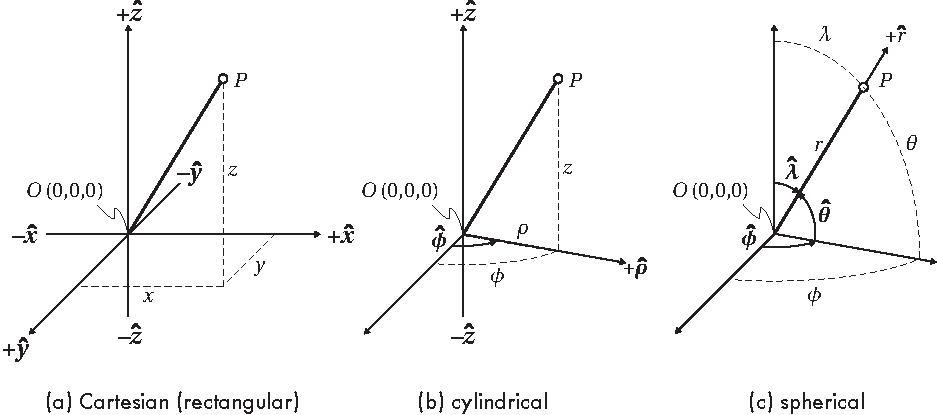
\includegraphics[]{math_primer/figures/coordinate_systems.pdf}
  }
  \caption{Commonly used coordinate systems. Axes labels with a $\hat{\ }$
  indicate a unit vector (vector of unit length).}
  \label{fig:coords}
\end{figure}

\section{Cartesian}
The first coordinate system to consider (and most familiar) is a {\it Cartesian
(rectangular) coordinate system} (Figure~\ref{fig:coords}a).  To describe our
space we will typically use the variables $x$, $y$, and $z$ and as a result each
point in space is defined by the coordinate triplet $(x,y,z)$.  In a Cartesian
system the principle axes (directions) are each orthogonal (at right angles) to
each other.

We will define our coordinate system such that it is right-handed.  To get an
intuitive feeling for what this means, take your right hand open with fingers
extended.  The direction your fingers point is the positive $x$-direction.  Now
keeping your fingers straight, bend your knuckles that join the fingers to the
palm.  Your palm and fingers should now form a right angle.  This is the
positive $y$-axis.  To determine the positive $z$-direction point your thumb out
away from your hand.  In geophysics we frequently choose the most convenient
coordinate system for our direction of interest.  If we are looking down into
the Earth for instance, we typically define the positive $z$-axis as down,
implying the cardinal directions $north$ and $east$ are the positive $x$- and
positive $y$-axes, respectively.  This definition of $+z$ down occasionally
reverses the sign of equations derived in physics, which has the amusing
side-effect of occasionally confuses physicists.  For short, we can identify
this coordinate system as NED, (north, east, down) = $(+x, +y, +z)$.

\section{Polar}
The polar coordinate system is a two-dimensional coordinate system that is
special case of cylindrical and spherical coordinates when $z = 0$ or $\theta =
0$, respectively.

Conversion from Cartesian $\leftrightarrow$\ polar:
\begin{align*}
    r &= (x^2 + y^2)^{1/2} & x &= r \cos \phi \\
    \phi &= \tan^{-1} \frac{y}{x} & y &= r \sin \phi \\
    \vu{r} &= \cos \phi \,\vu{x} + \sin \phi \,\vu{y} &
    \,\vu{x} &= \cos \phi \,\vu{r} - \sin \phi \,\vu{\phi} \\
    \vu{\phi} &= -\sin \phi \,\vu{x} + \cos \phi \,\vu{y} &
    \,\vu{y} &= \sin \phi \,\vu{r} + \cos \phi \,\vu{\phi} \\
\end{align*}

\section{Cylindrical}
We may also define a {\it cylindrical coordinate system} which we define as $\rho$, $\phi$, and $z$ (Figure~\ref{fig:coords}b).  Imagine a circular cylinder with the $z$-direction forming the axis of the cylinder.  The cross-section of the cylinder defines a circle with radius $\rho$.  The third coordinate is an angle $\phi$ defined clockwise in the plane of the cylinder's cross section.  Systems which are cylindrically symmetric are called axially symmetric and variations are typically described in terms of the axial ($z$) direction and radial direction (cross-section of the cylinder).  Note: because the radius is defined differently for the cylindrical and spherical coordinate systems, we use $\rho$ for the radius in cylindrical coordinates to differentiate it from $r$ used in spherical coordinates.

Conversion from Cartesian $\leftrightarrow$\ cylindrical:
\begin{align*}
    \rho &= (x^2 + y^2)^{1/2} & x &= \rho \cos \phi \\
    \phi &= \tan^{-1} \frac{y}{x} & y &= \rho \sin \phi \\
    z &= z & z &= z \\
    \vu{r} &= \cos \phi \,\vu{x} + \sin \phi \,\vu{y} &
    \vu{x} &= \cos \phi \,\vu{r} - \sin \phi \,\vu{\phi} \\
    \vu{\phi} &= -\sin \phi \,\vu{x} + \cos \phi \,\vu{y} &
    \vu{y} &= \sin \phi \,\vu{r} + \cos \phi \,\vu{\phi} \\
    \vu{z} &= \,\vu{z} & \,\vu{z} &= \,\vu{z}
\end{align*}

\section{Spherical}
A third coordinate system commonly used in geophysics is a {\it spherical
coordinate system} (Figure~\ref{fig:coords}c). Points within this system are
defined by the radius of a sphere $r$ and two angles that describe where $r$
points.  One angle about the equator (longitude), $\phi$, defined counter
clockwise and the second is defined from the north pole to south pole
(co-latitude), $\theta$.  For many Earth applications, we use the latitude as an
angle defined from the equator to the pole, $\lambda$, where the latitude is
related to the co-latitude by $\lambda = 90 - \theta$ in degrees.  Systems which
are spherically symmetric are described in terms of a radial direction only.

Conversion from Cartesian $\leftrightarrow$ spherical:
\begin{align*}
    r &= (x^2 + y^2 + z^2)^{1/2} & x &= r \sin \theta \cos \phi \\
    \theta &= \cos^{-1} \frac{z}{r} & y &= r \sin \theta \sin \phi \\
    \phi &= \tan^{-1} \frac{y}{x} & z &= r \cos \theta \\
    \vu{r} &= \sin \theta \cos \phi \,\vu{x} + \sin \theta \sin \phi
        \,\vu{y} + \cos \theta \,\vu{z} &
    \vu{x} &= \sin \theta \cos \phi \,\vu{r} + \cos \theta \cos \phi
        \,\vu{\theta} - \sin \phi \,\vu{\phi} \\
    \vu{\theta} &= \cos \theta \cos \phi \,\vu{x} + \cos \theta \sin \phi
        \,\vu{y} - \sin \theta \,\vu{z} &
    \vu{y} &= \sin \theta \sin \phi \,\vu{r} + \cos \theta \sin \phi
        \,\vu{\theta} + \cos \phi \,\vu{\phi} \\
    \vu{\phi} &= \sin \phi \,\vu{x} + \cos \phi \,\vu{y} &
    \vu{z} &= \cos \theta \,\vu{r} - \sin \theta \,\vu{\theta}
\end{align*}

Conversion from cylindrical $\leftrightarrow$ spherical:
\begin{align*}
    r &= (\rho^2 + z^2)^{1/2} & x &= r \cos \phi \\
    \theta &= \tan^{-1} \frac{\rho}{z} = \cos^{-1} \frac{z}{r} &
        y &= r \sin \phi \\
    \phi &= \phi & z &= z \\
    \vu{r} &= \sin \theta \,\vu{\rho} + \cos \theta \,\vu{z} &
    \vu{\rho} &= \sin \theta \,\vu{r} + \cos \theta \,\vu{\theta} \\
    \vu{\theta} &= \cos \theta \,\vu{\rho} - \sin \theta \,\vu{z} &
    \vu{z} &= \cos \theta \,\vu{r} - \sin \theta \,\vu{\theta} \\
    \vu{\phi} & = \,\vu{\phi} & \,\vu{\phi} &= \,\vu{\phi}
\end{align*}

\section{Derivatives}

\section{Integrals}
Suppose we wanted to take an integral along a path or about an area or volume but we wish to change coordinate systems to simplify the math.  In this case we have to change the infintesimal.  In the case of a line integral,
\begin{equation*}
    \dd{\ell} = 
    \begin{cases}
        \vu{x} \dd{x} + \vu{y} \dd{y} + \vu{z} \dd{z} & \text{Cartesian} \\
        \vu{\rho} \dd{\rho} + \vu{\phi} \rho \dd{\phi} + \vu{z} \dd{z} &
            \text{cylindrical} \\
        \vu{r} \dd{r} + \vu{\theta} r \dd{\theta} + \vu{\phi} r \sin
            \theta \dd{\phi} & \text{spherical}\\
    \end{cases}
\end{equation*}
Integrals over area do not have a simple conversion in the same way because it
depends on the direction of the point to the origin.

For a volume integral,
\begin{equation*}
    \dd{v} =
    \begin{cases}
        \dd{x} \dd{y} \dd{z} & \text{Cartesian} \\
        \rho \dd{\rho} \dd{\phi} \dd{z} & \text{cylindrical} \\
        r^2 \sin \theta \dd{r} \dd{\theta} \dd{\phi} & \text{spherical} \\
    \end{cases}
\end{equation*}
